\documentclass[12pt]{extarticle}

\usepackage[utf8]{inputenc}
\usepackage[hungarian=nohyphenation]{hyphsubst}
\usepackage[hungarian]{babel}
\usepackage{graphicx}
\usepackage{subcaption}
\usepackage{fancyhdr}
\usepackage{caption}
\usepackage{url}
\usepackage{siunitx}
\usepackage{amsmath}
\usepackage{pdfpages}

\title{\huge Mikrovezérlők projekt feladat\\[10pt]
	\Large LED-sor vezérlés}
\date{\today}
\author{Máté Bálint, Pádár Gergely, Tar Dániel }


\begin{document}
	
	\begin{titlepage}
		\lhead{
\includegraphics[height=2cm]{logo_mogi.png}}
		\rhead{\large{\textbf{Mikrovezérlők alkalmazása}}\\
			\large{BMEGEFOAMV1}}
		
		\maketitle
		\pagenumbering{gobble}
		\thispagestyle{fancy}
		
		\begin{figure}
			\begin{center}
				
\includegraphics[height=2cm]{logo_bme_kicsi.eps}
			\end{center}
		\end{figure}
		
	\end{titlepage}
	
	
	\newpage
	\pagenumbering{gobble}
	\tableofcontents
	
	
	\newpage
	\pagenumbering{arabic}
	
	
	\section{Feladat ismertetése}
	
	LED-sor színének beállítása mikrokontrollerrel. Majd vezeték nélküli vezérlés megoldása wi-fi modul segítségével. Továbbá felhasználóbarát Android alkalmazással a LED-ek színének beállítása egy egyszerű GUI-n.
	
	\begin{figure}[h!]
		\centering
		\begin{subfigure}[b]{0.3\linewidth}
			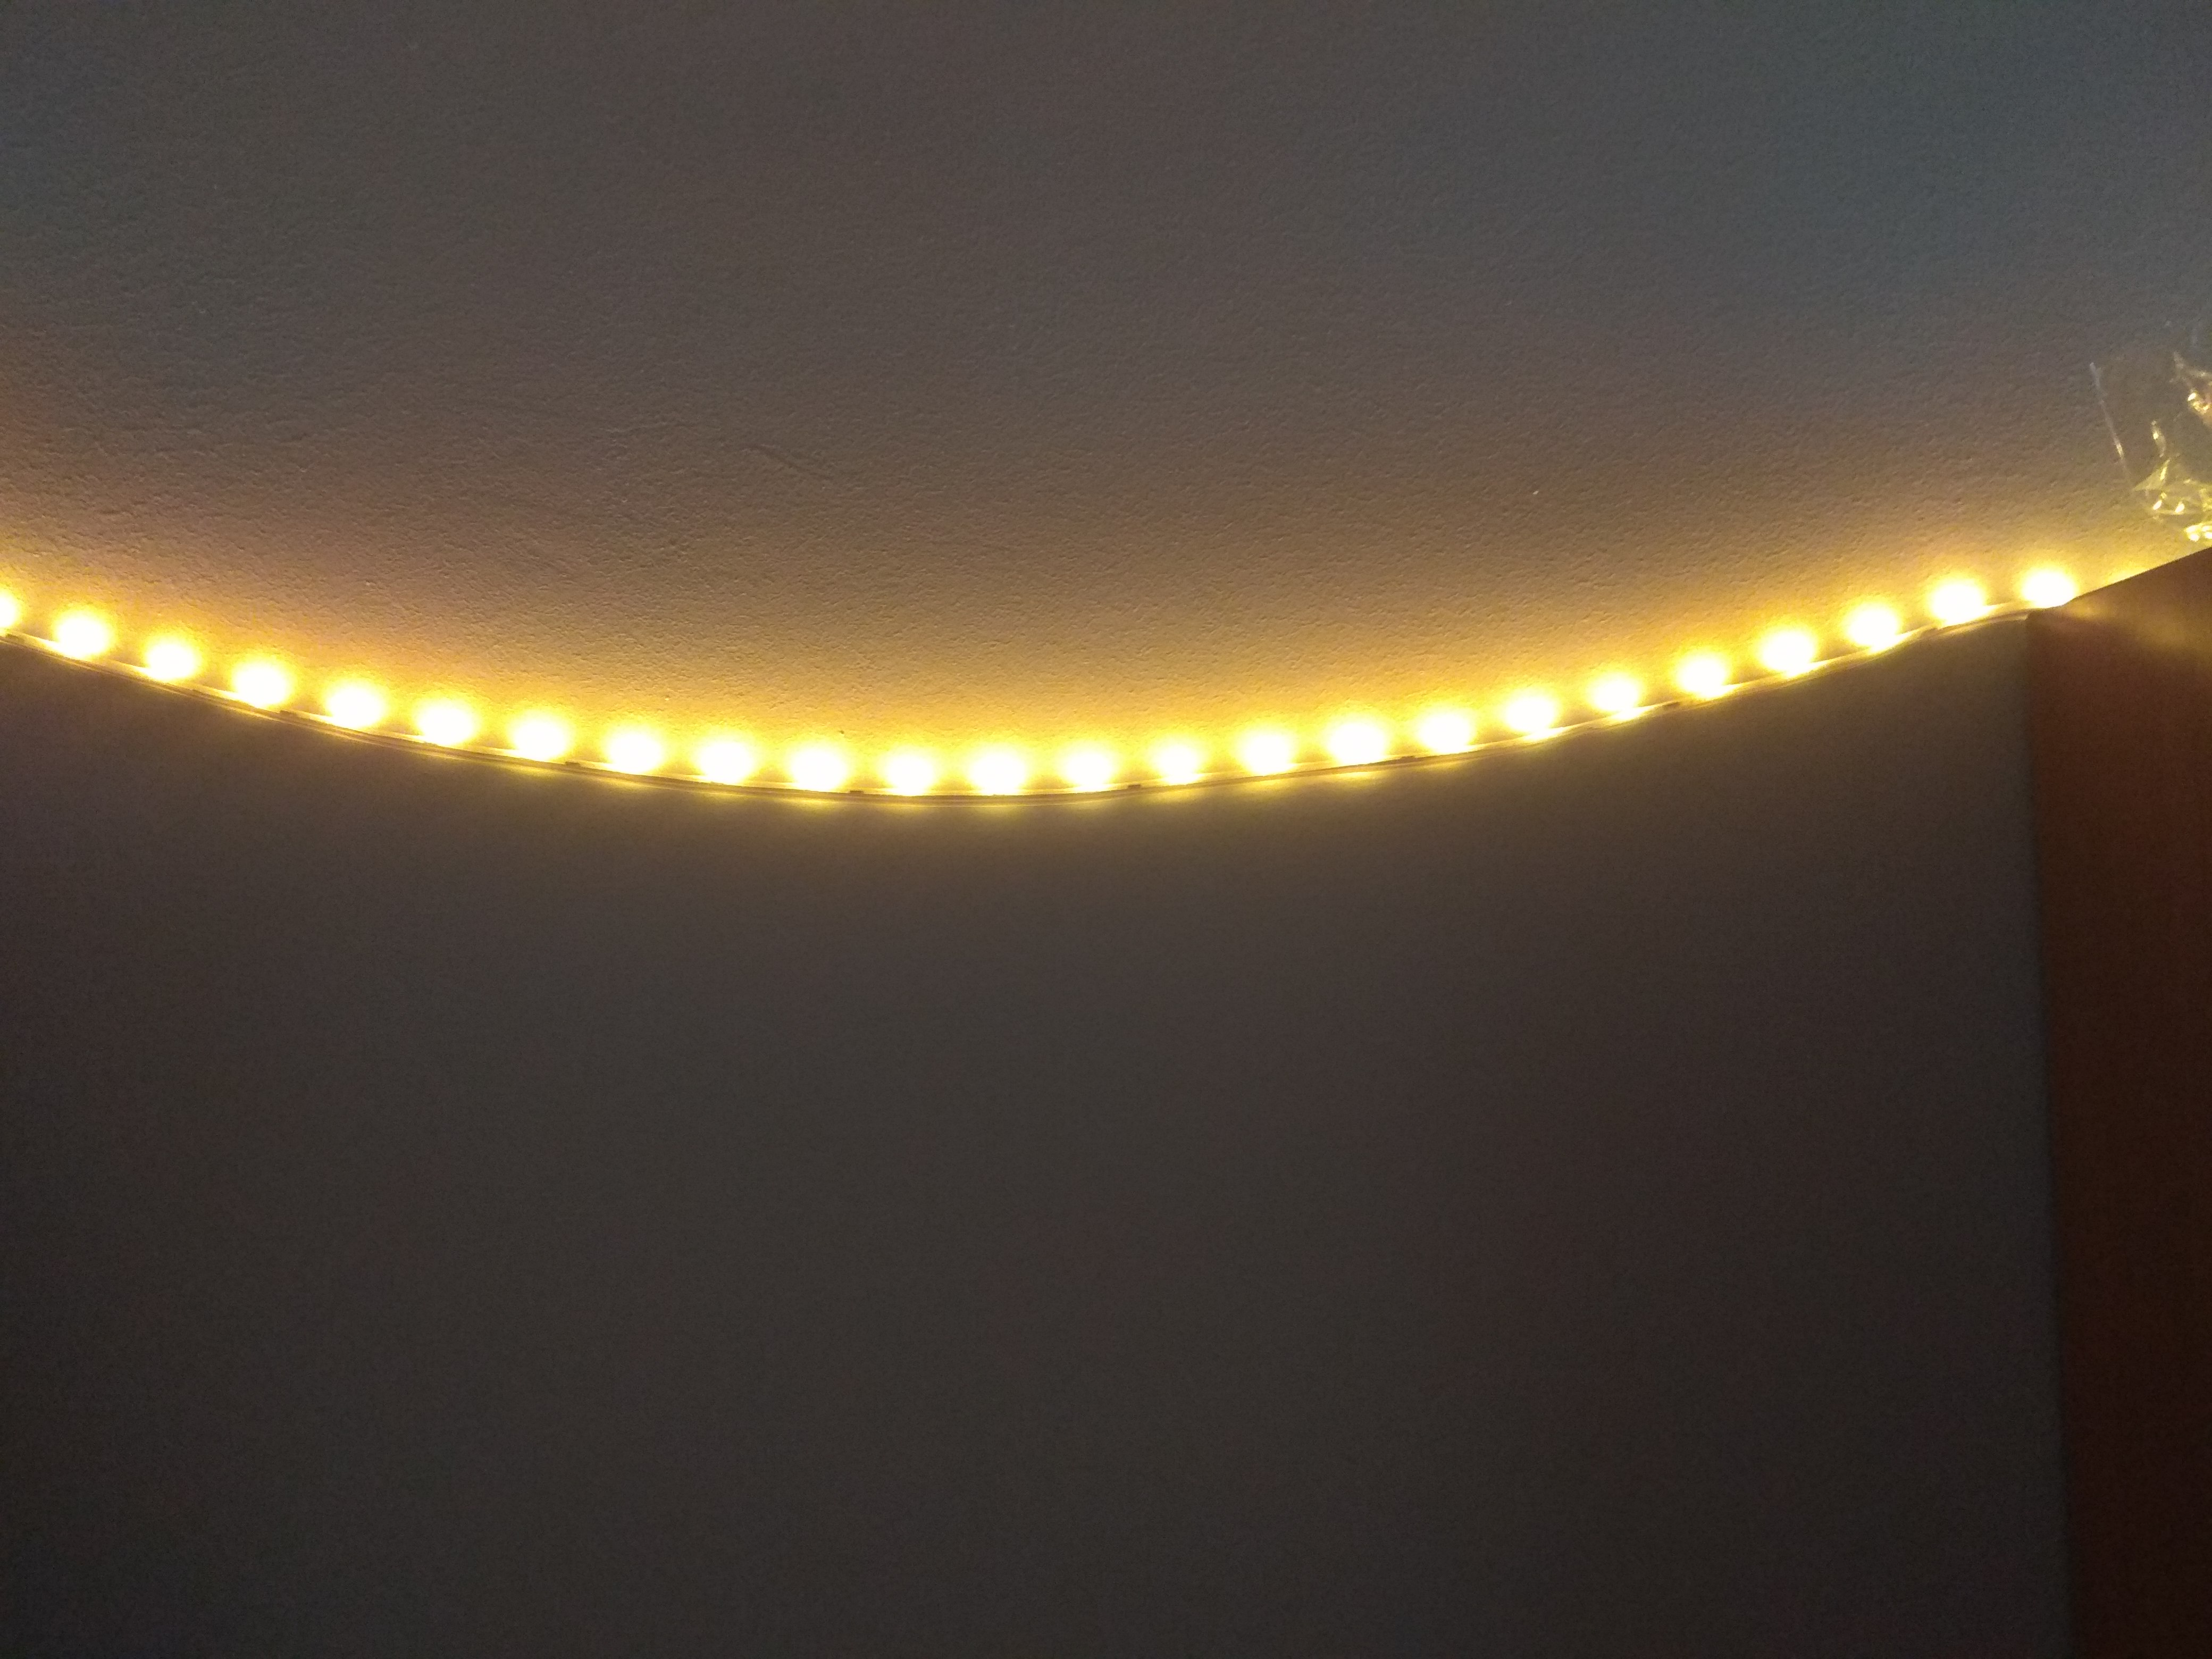
\includegraphics[width=\linewidth]{sarga.jpg}
			\caption{Narancssárga}
		\end{subfigure}
		\begin{subfigure}[b]{0.3\linewidth}
			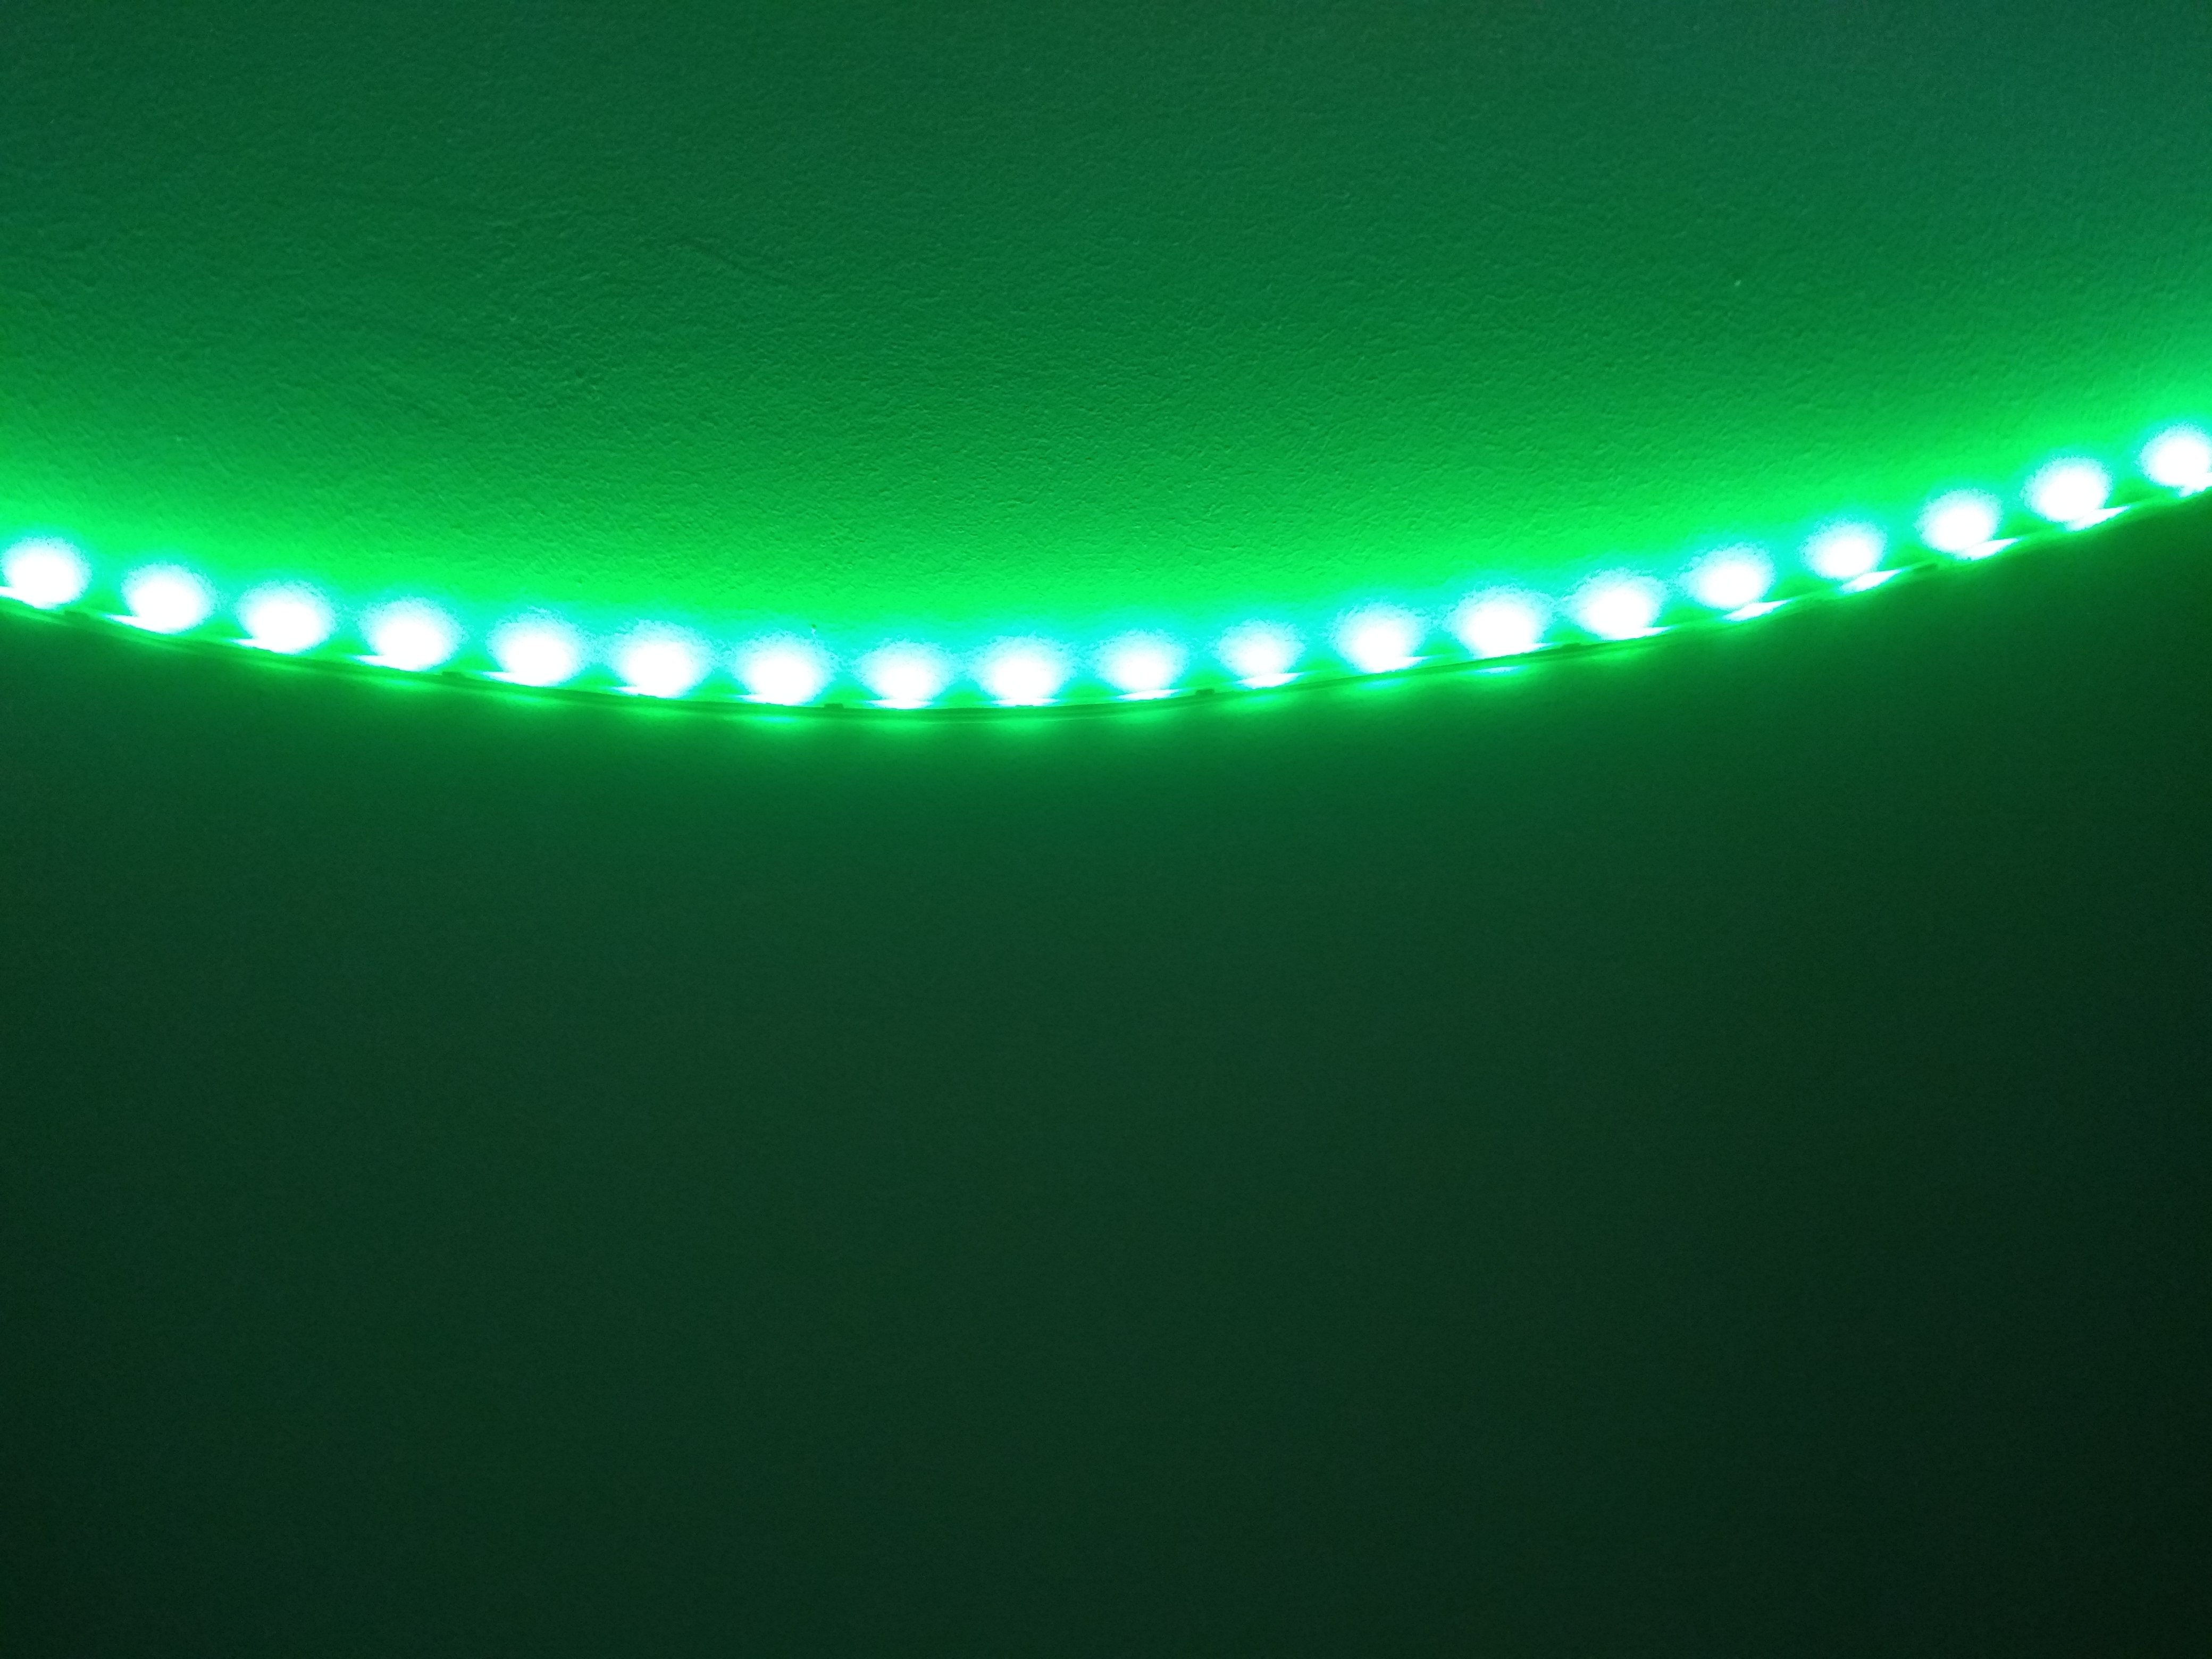
\includegraphics[width=\linewidth]{zold.jpg}
			\caption{Zöld}
		\end{subfigure}
		\begin{subfigure}[b]{0.3\linewidth}
			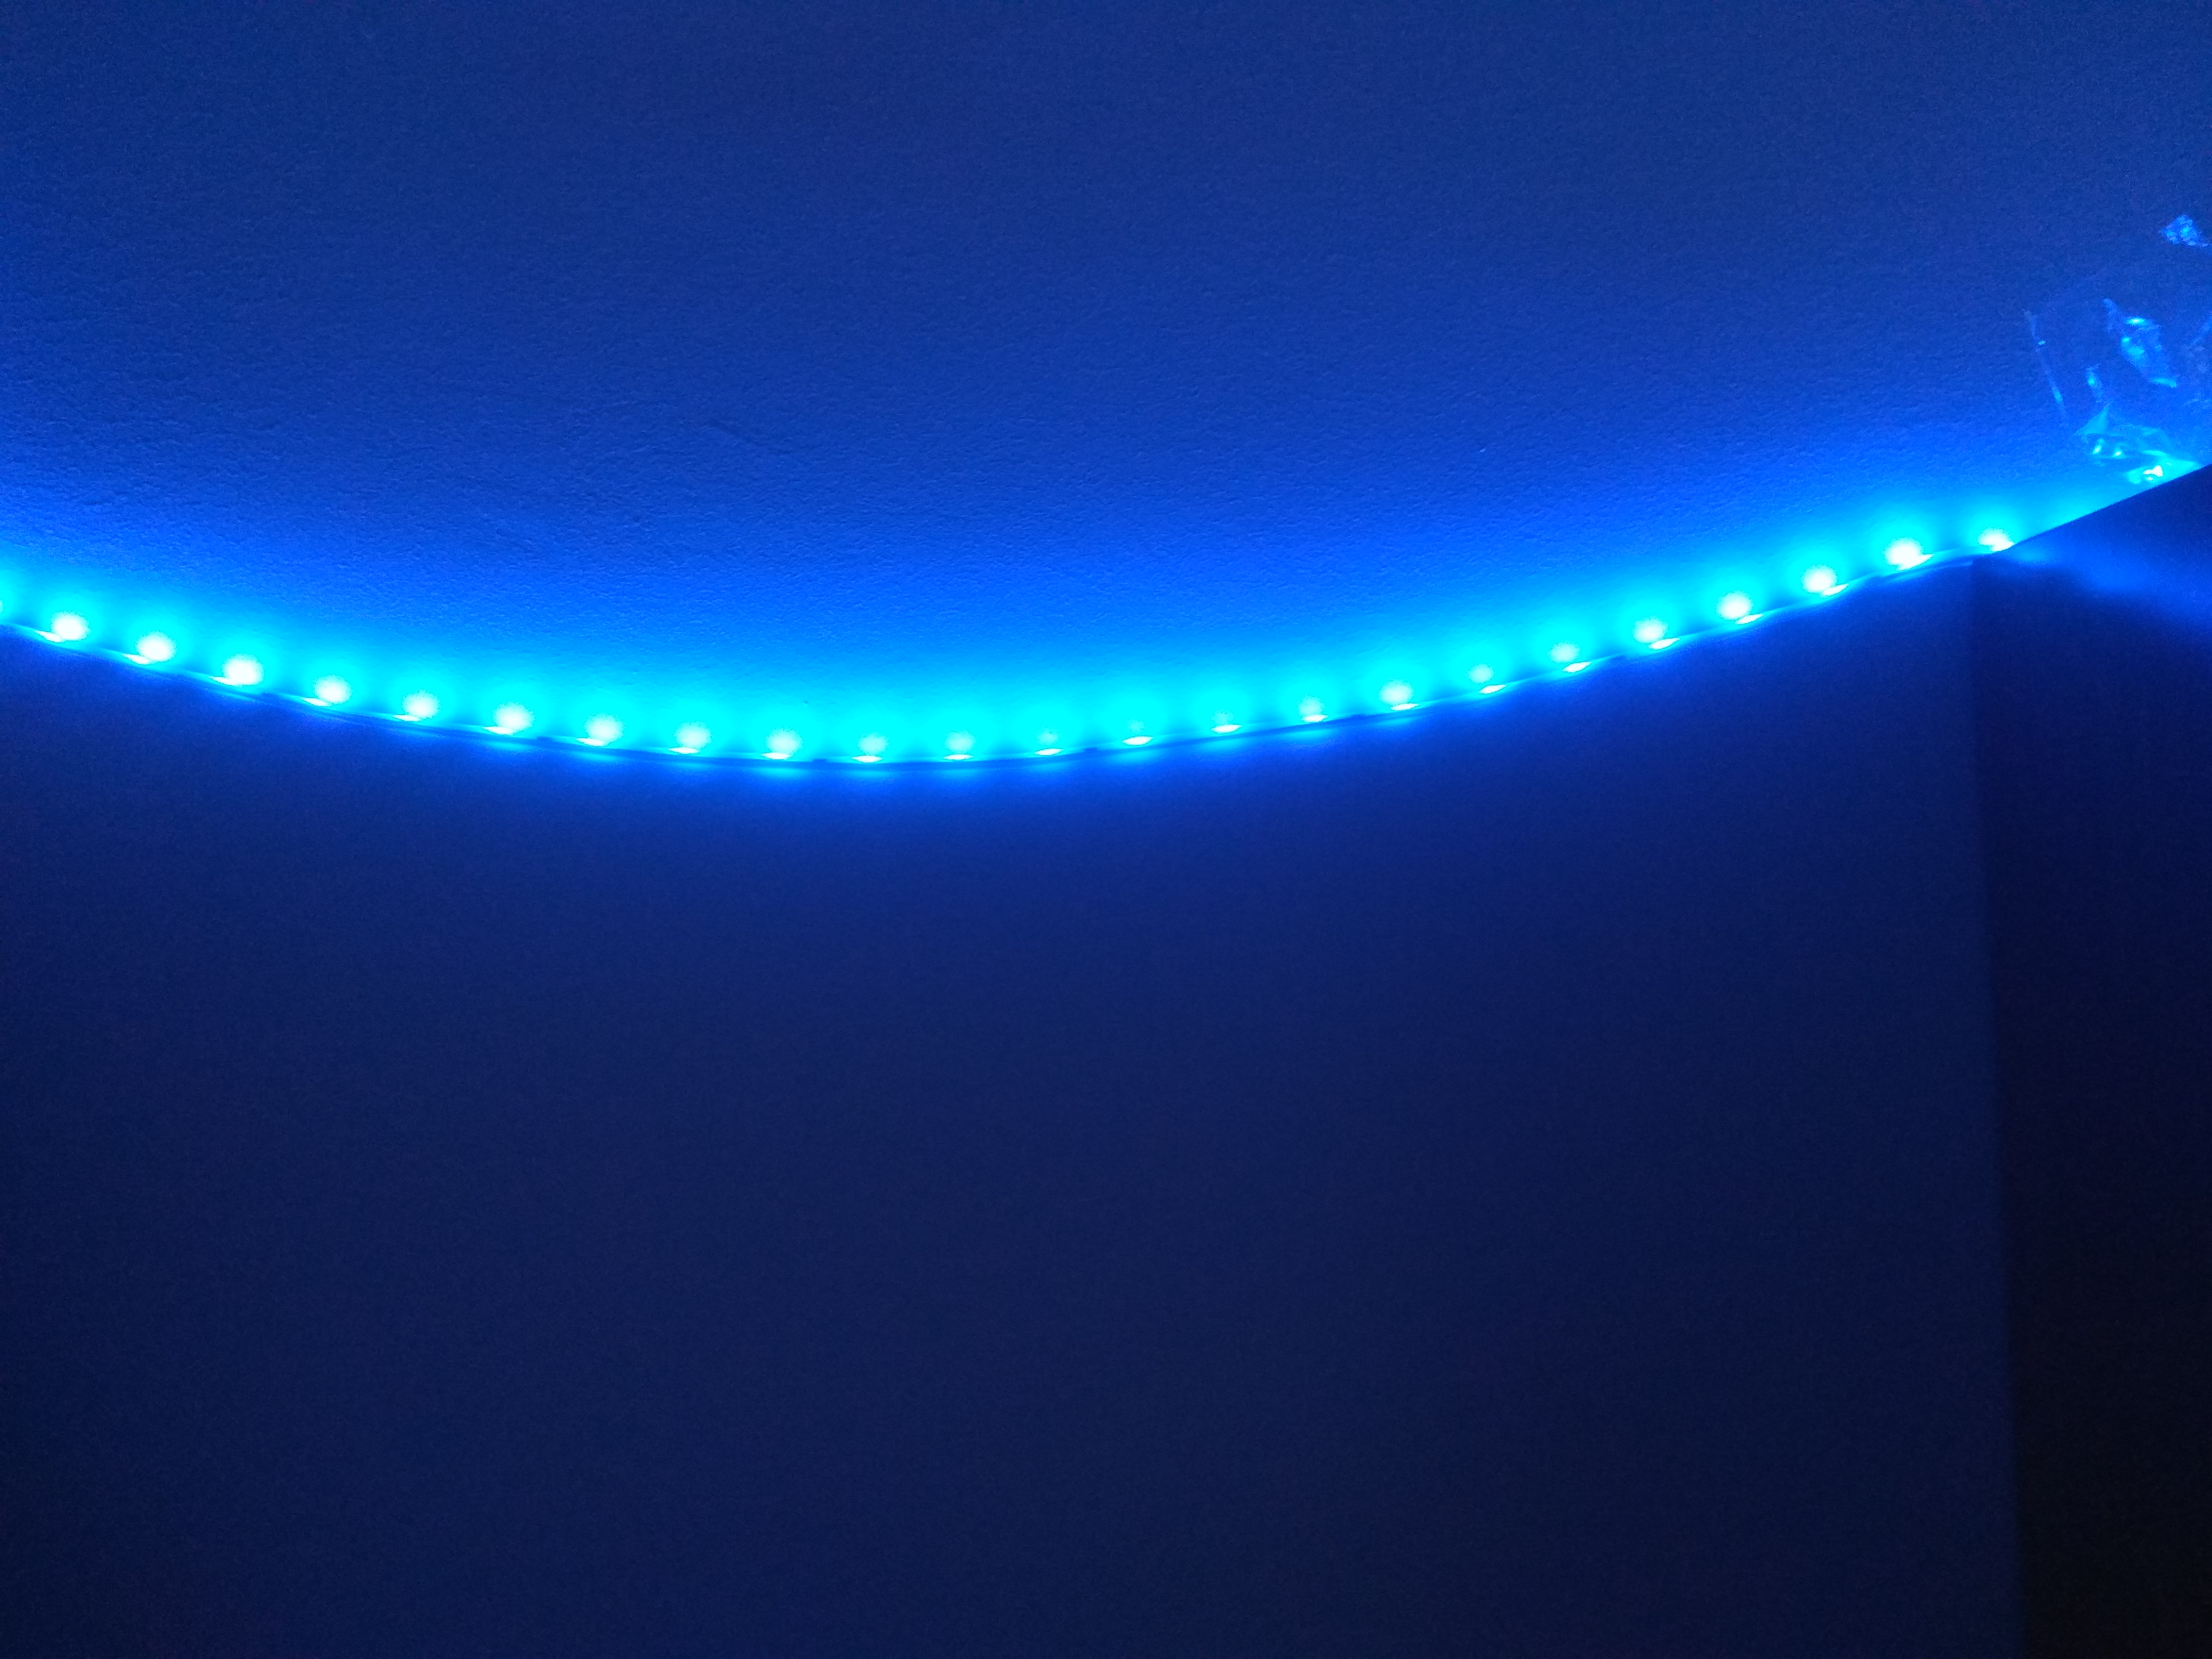
\includegraphics[width=\linewidth]{kek.jpg}
			\caption{Kék}
		\end{subfigure}
		\caption{A világító LED-sor}
		\label{}
	\end{figure}

	\begin{figure}[h!]
		\centering
		\begin{subfigure}[b]{0.3\linewidth}
			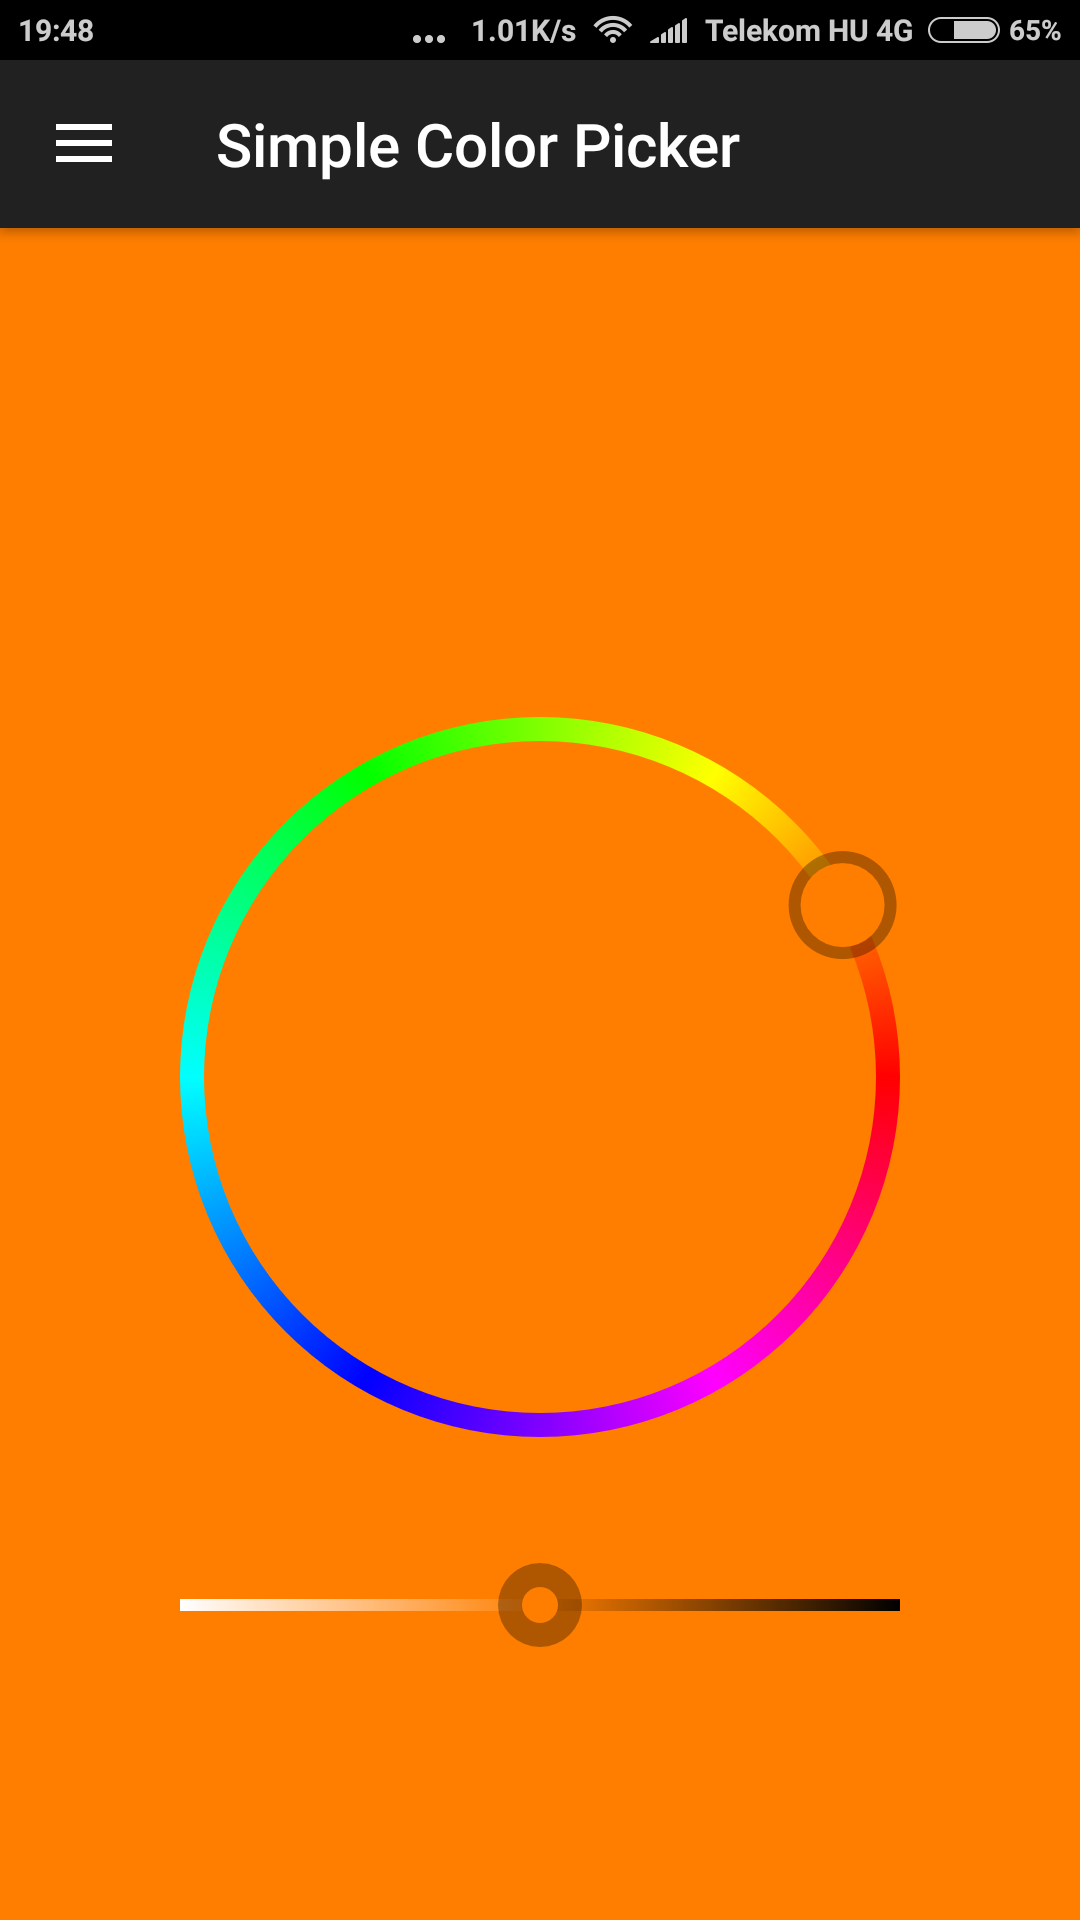
\includegraphics[width=\linewidth]{sarga2.png}
			\caption{Narancssárga}
		\end{subfigure}
		\begin{subfigure}[b]{0.3\linewidth}
			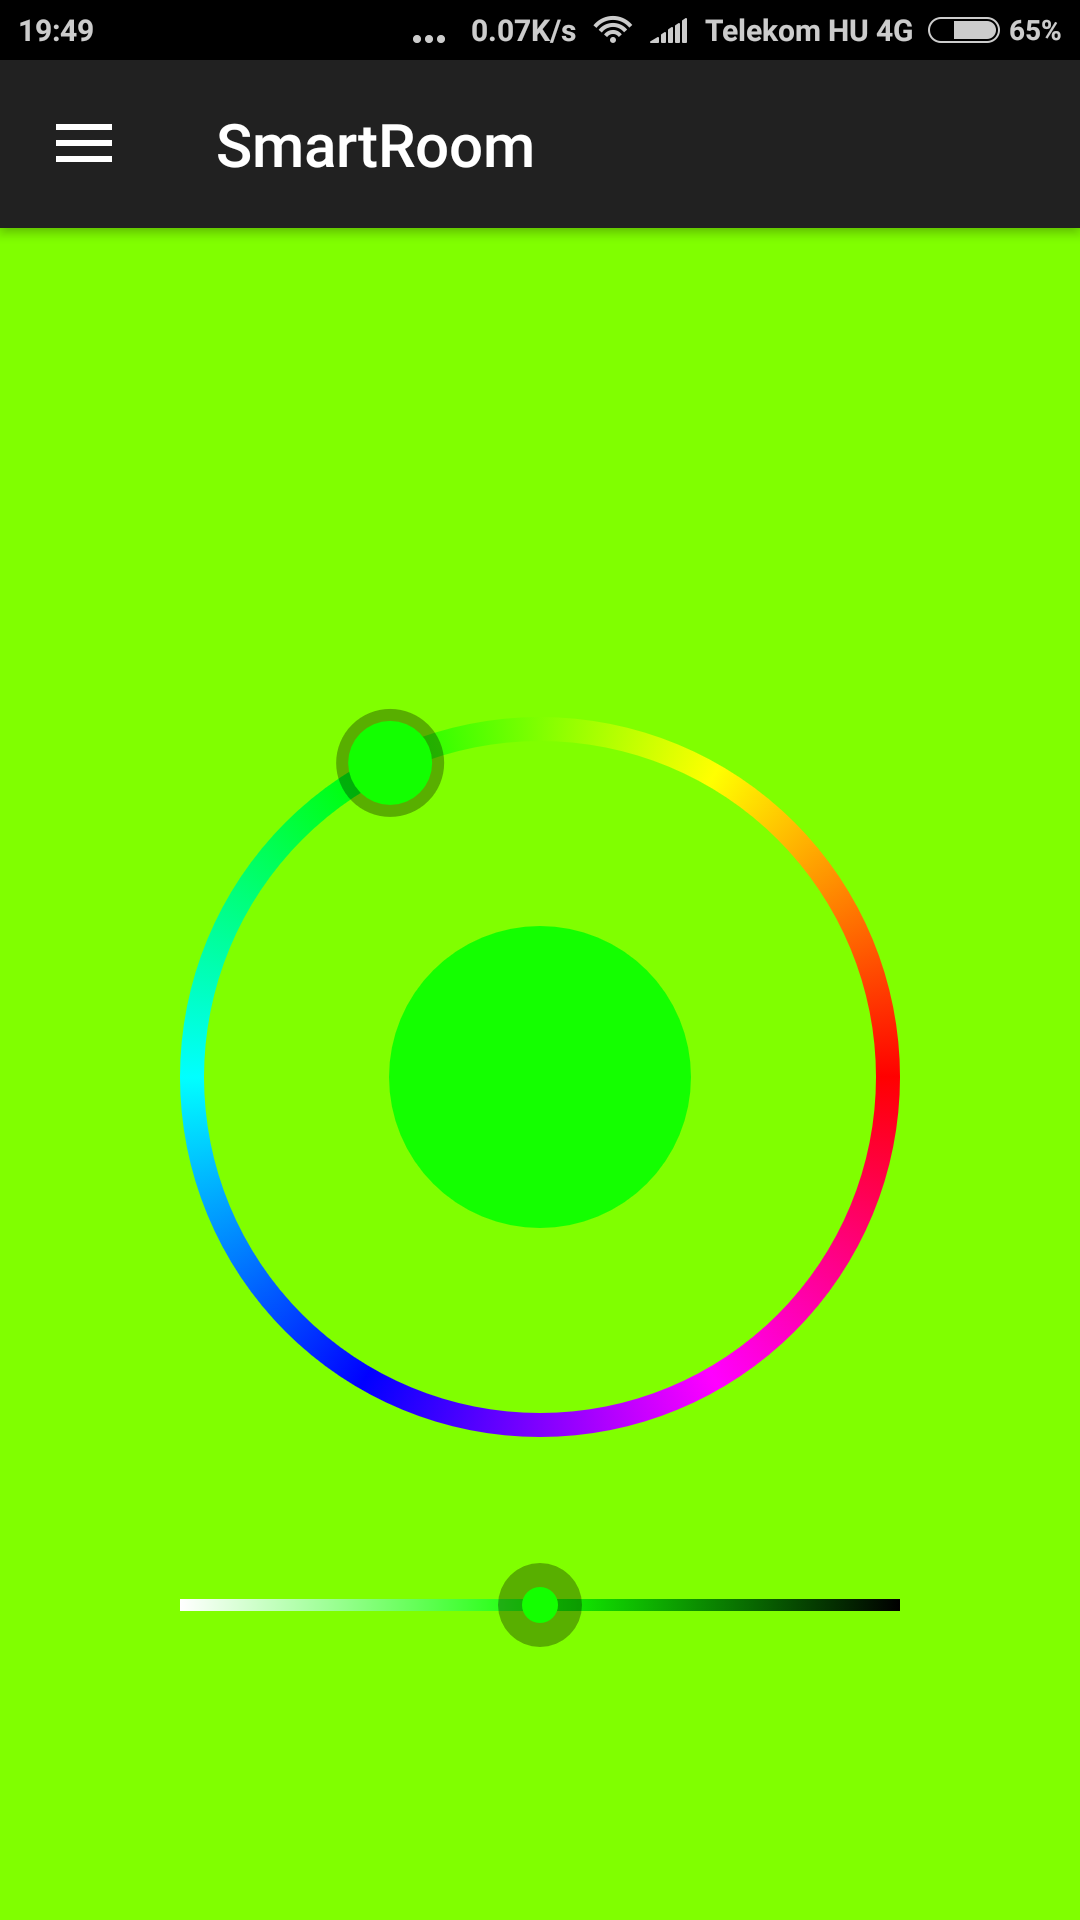
\includegraphics[width=\linewidth]{zold2.png}
			\caption{Zöld}
		\end{subfigure}
		\begin{subfigure}[b]{0.3\linewidth}
			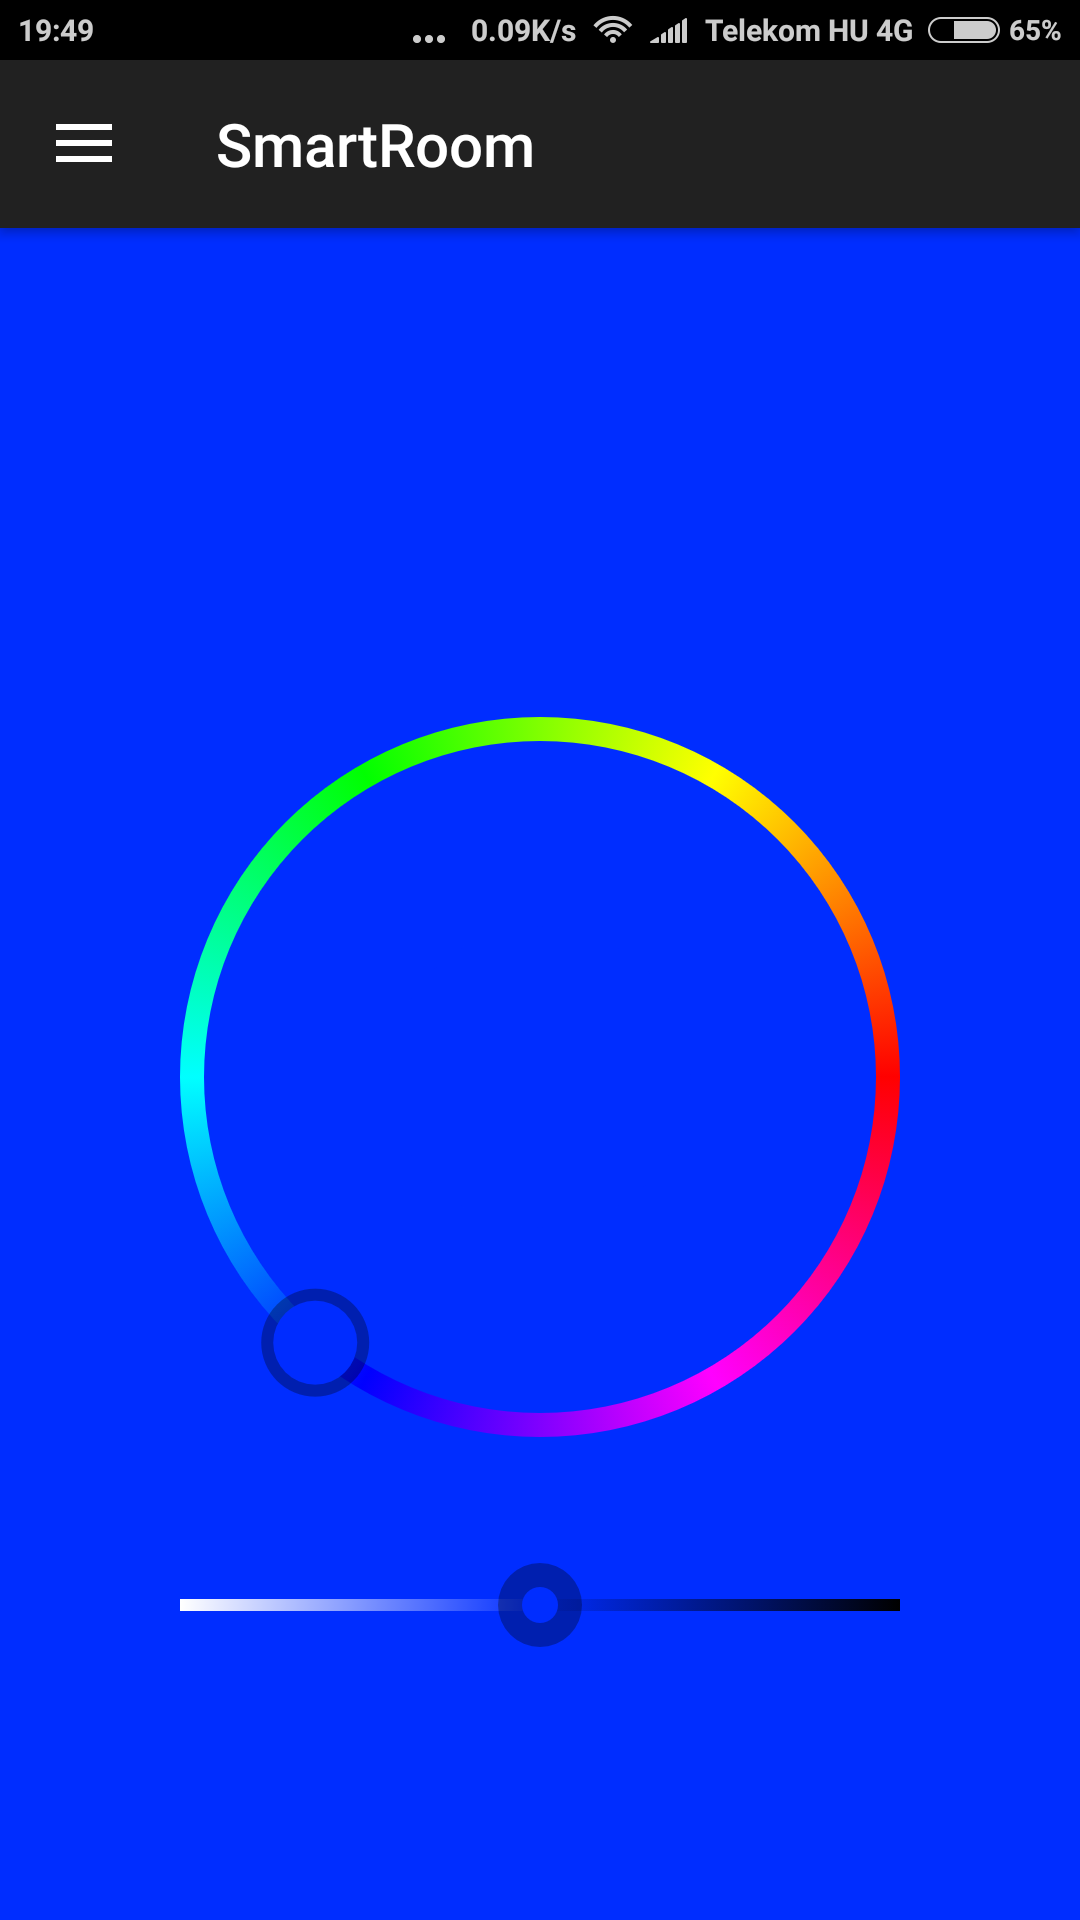
\includegraphics[width=\linewidth]{kek2.png}
			\caption{Kék}
		\end{subfigure}
		\caption{A szín beállítása csúszkával az Android alkalmazás felhasználói felületén}
		\label{}
	\end{figure}


	
	\section{Megoldás részletezése}
	
	\begin{itemize}
		\item 	Az android alkalmazásnál beállítható a vezérelendő eszköz IP címe a \ref{ip}. ábrán látható módon 
		
		\begin{figure}[h!]
			\centering
			\begin{subfigure}[b]{0.4\linewidth}
				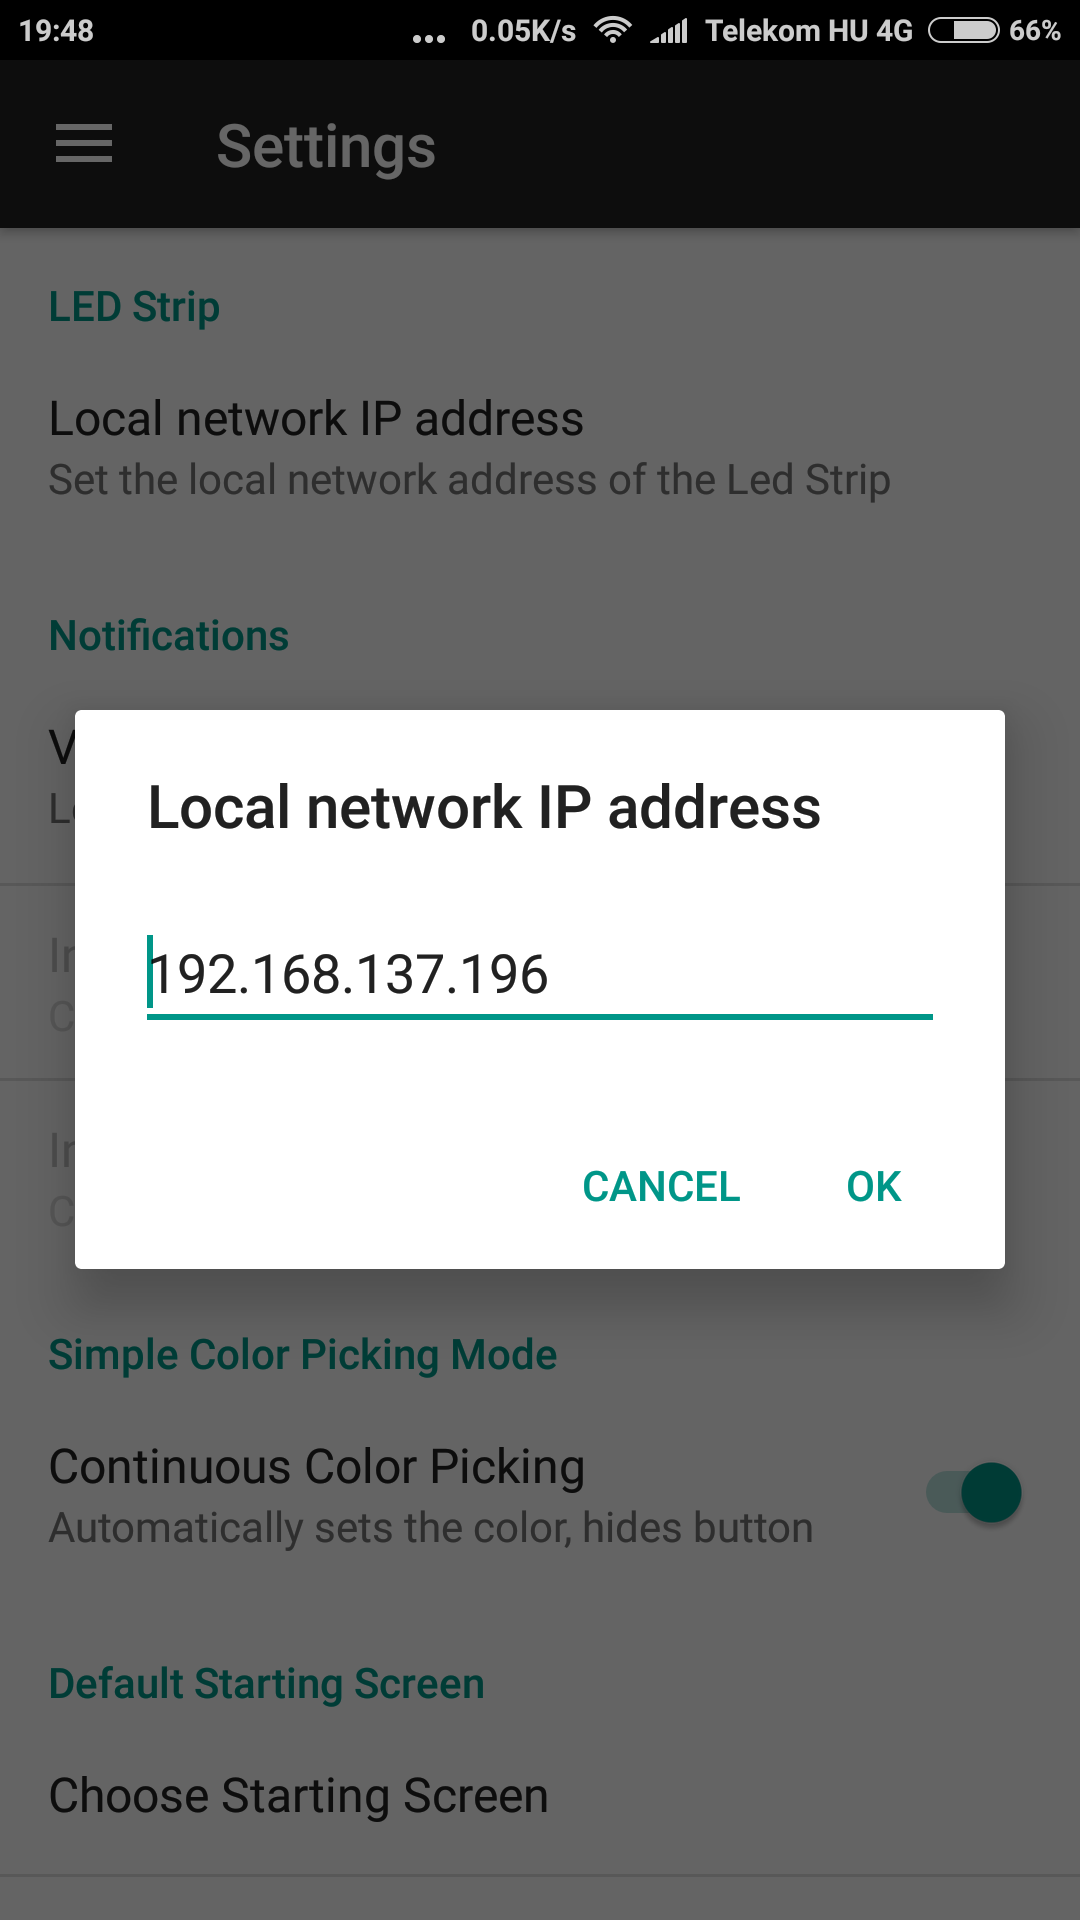
\includegraphics[width=\linewidth]{ip.png}
				\caption{}
			\end{subfigure}
			\begin{subfigure}[b]{0.4\linewidth}
				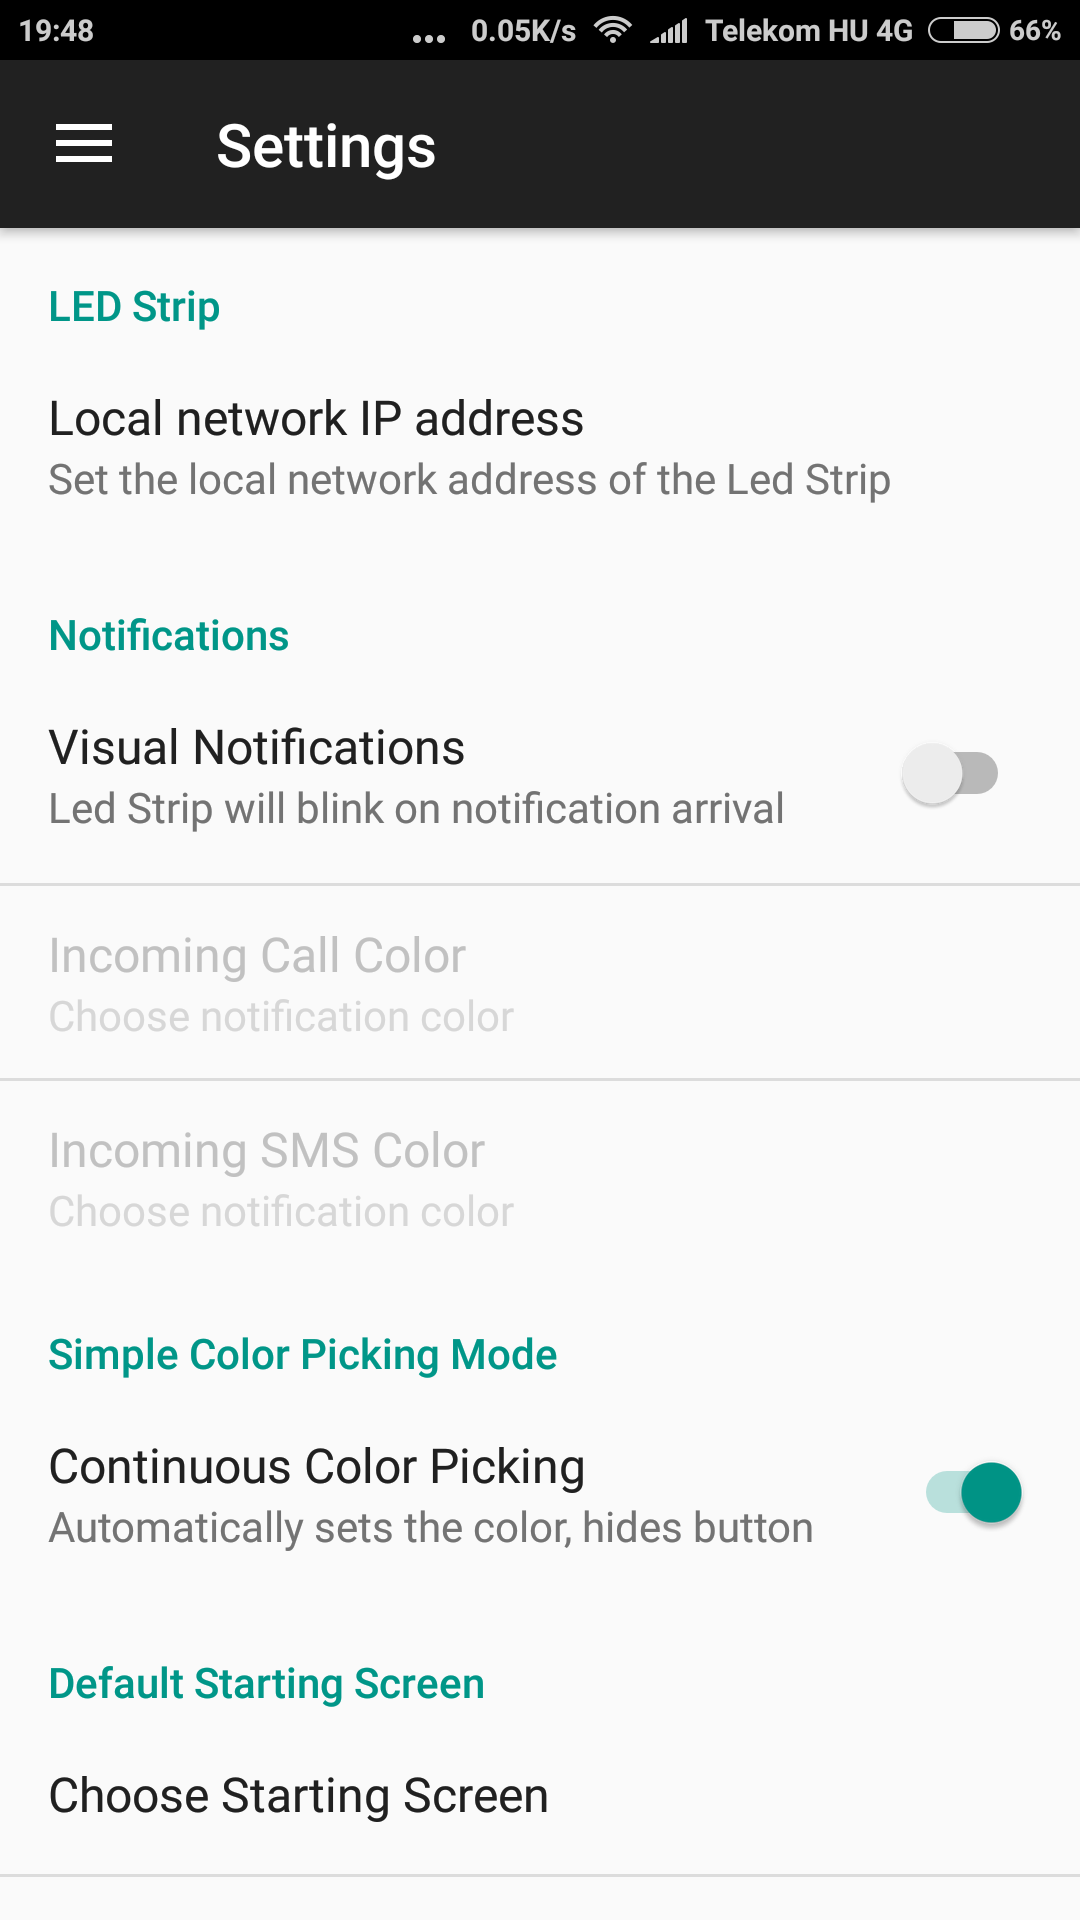
\includegraphics[width=\linewidth]{ip2.png}
				\caption{}
			\end{subfigure}
			\caption{Az Wifi modul IP címének beállítása az Android applikációban}
			\label{ip}
		\end{figure}
	
	
		
		\item Ezután UDP csomagokat küldünk a céleszközre RGBM felosztásban, ahol R,G,B a vörös, zöld és kék színek 8 bites erősségét, az M pedig a moduláció mértékét jelenti
		
		\item A wi-fi modul a beérkező csomagokat fogadja
		
		\item A beérkezett adatok a következő formátumban lesznek UART soros kommunikáción keresztül továbbküldve a mikrokontrollernek:
		
		\begin{equation*}
			+IPD,<len>:<data>
		\end{equation*}
		
		Ahol len az érkező adat hosszát jelenti bájtban, data pedig magát az adatot jelöli.
		
		\item A mikrokontroller a beérkező adatcsomagot lementi egy adott memória területre

		\item Végül a fő ciklusban a LED-sor által értelmezhető formátumban küldi tovább.
		
	\end{itemize}
	
	
		
	
	\section{Felhasznált eszközök}
	
	A szükséges eszközöket eBay-ről szereztük be. A LED-sor kb. 3500 Ft, a mikrovezérlő kb. 650 Ft, a wifi modul kb. 600 Ft, a DC/DC konverter pedig kb. 400 forintba került. Tehát az egész projekthez szükséges elektronika 5500 Ft-ból beszerezhető.
	
	\subsection{LED-sor}
	
	A LED-sor egy szegmense 3 db RGB LED-ből, valamint egy  WS2811 típusú IC-ből áll. Az 5 méter hosszú soron 50 db ilyen szegmens helyezkedik el.  
	
	\subsection{Mikrovezérlő}
	
	A feladathoz az egyik legelterjedtebb, egy STM32F103C8 típusú mikrokontrollert használtunk. 
	
	\subsection{Wi-fi modul}
	
	Ide egy ESP8266 számú modult szeretünk be.
	
	\subsection{DC/DC konverter}
	
	A DC/DC stepdown konvertert a mikrokontrollernek és wifi modulnak megfelelő 3.3V-os feszültség (5V lenne az ideális a WS2811 signal lábához, de így is működőképes) előállítására használjuk 
	
	
	
	
	
	
	
	
	
	
	
	
	
	
	
	
	
\end{document}